\chapter{Implementation}
\label{implementation}
In diesem Kapitel wird die Konzeption des Brute Force-Angriffs beschrieben. Auf Basis der beschriebenen Konzeption wird im Anschluss die Implementation erfolgen. 
\section{Nachrichtenstruktur}
Da unsere Implementation auf einer nachrichtenbasierten Kommunikation basieren wird, ist der Entwurf eigener Nachrichtenstrukturen notwendig. Die Nachrichtenstrukturen übertragen alle projektrelevanten Informationen zwischen dem Master und dem Worker oder den Workern. Zur Strukturierung fiel die Wahl auf das Nachrichtenaustauschformat \enquote{JavaScript Object Notation} oder kurz \emph{JSON}, da dieses Format sehr leichtgewichtig und sehr gut anpassbar ist. \\
%TODO WORKER_ID == Hostname/IP
Nachfolgend werden die entwickelten Nachrichtenstrukturen und deren Inhalt detailliert beschrieben. Dabei wird zwischen \emph{Basic Messages} und \emph{Extended Messages} unterschieden. 
%TODO Basic und extended Messages erklären

\subsubsection{Basic Messages}
Hier werden die Strukturen beschrieben, welche vom steuernden Rechner (Master) zu einem der Worker gesendet werden.\\

\texttt{SetupAndConfig}
\begin{lstlisting}[basicstyle=\ttfamily,numbers=left,numberstyle=\footnotesize\ttfamily,backgroundcolor=\color{sourcegray}]
{
  "status" : "setupConfig",
  "value" : {
    "algorithm" : "#HASH_ID",
    "target" : "#TARGET_HASH", 
    "worker_id" : "#WORKER_ID"
  }
}
\end{lstlisting}
Ein im Cluster neu hinzugefügter Worker erhält seine Konfigurationsparameter, damit dieser mit dem Berechnen beginnen kann. 
Der Wert \textbf{algorithm} übergibt die ID des Hash-Algorithmus, welcher in der aktuellen Passwortberechnung benutzt wird. \textbf{Target} übermittelt den Hash des Zielpasswortes. Anhand des Hashes kann ein Worker bestimmen, ob das Zielpasswort berechnet wurde. Die \textbf{workerID} ist eine vom Master vergebene, fortlaufende Nummer und dient der Identifizierung der Worker.\\

\texttt{getWork}
\begin{lstlisting}[basicstyle=\ttfamily,numbers=left,numberstyle=\footnotesize\ttfamily,backgroundcolor=\color{sourcegray}]
{
  "status" : "newWorkBlog",
  "value" : {
    "worker_id" : "#WORKER_ID"
    "hashes" : ["#NEW_HASHES"]
  }
}\end{lstlisting}
Diese Nachricht übermittelt dem Worker eine Anzahl neuer Passwörter, von denen dieser die Hashes berechnen wird.\\
 %TODO Beschreibung fertigstellen.

\texttt{stillAlive}
\begin{lstlisting}[basicstyle=\ttfamily,numbers=left,numberstyle=\footnotesize\ttfamily,backgroundcolor=\color{sourcegray}]
{
  "status" : "stillAlive",
  "value" : ""
}
\end{lstlisting}
Mit Hilfe dieser Nachricht fragt der Master an, ob die angesprochenen Worker noch verfügbar sind. Wenn diese nicht antworten, werden sie aus dem Array der verfügbaren Worker entfernt.


\subsubsection{Extended Messages}
Folgende Nachrichten werden von den Workern an die Master gesendet. \\

\texttt{newClientRegistration}
\begin{lstlisting}[basicstyle=\ttfamily,numbers=left,numberstyle=\footnotesize\ttfamily,backgroundcolor=\color{sourcegray}]
{
  	"status" : "newClientRegistration",
	"worker" : "#WORKER_ID"
}
\end{lstlisting}
Der Worker beantragt eine ID, um sich im Cluster identifizieren zu können.\\

\texttt{hitTargetHash}
\begin{lstlisting}[basicstyle=\ttfamily,numbers=left,numberstyle=\footnotesize\ttfamily,backgroundcolor=\color{sourcegray}]
{
  "status" : "hitTargetHash",
  "value" : {
    "hash" : "#HASH_VALUE",
    "password" : "#PASSWORD"
    "time_needed" : "#TIME"
    "worker_id" : "#WORKER_ID"
  }
}\end{lstlisting}
Diese Nachricht wird vom Worker versendet, wenn der berechnete Hash dem Zielhash entspricht und somit das Passwort berechnet wurde. Es werden der berechnete Hash und das zugehörige Passwort übertragen. Zudem wird die Zeit, die die Berechnung in Anspruch genommen hat, übertragen. Die Zeit kann für spätere Erweiterungen des Projekts genutzt werden, beispielsweise zum Vergleich verschiedener Hash-Algorithmen.\\
%TODO Beschreibung fertigstellen.

\texttt{finishedWork}
\begin{lstlisting}[basicstyle=\ttfamily,numbers=left,numberstyle=\footnotesize\ttfamily,backgroundcolor=\color{sourcegray}]
{
  "status" : "finishedWork",
  "value" : "#WORKER_ID"
}
\end{lstlisting}
Mit dieser Nachricht teilt der Worker mit, dass alle möglichen Passworte des aktuellen Arbeitspakets berechnet worden sind. Falls bei der Berechnung der Zielhash bzw. das Zielpasswort berechnet worden ist, wird zusätzlich die Nachricht \enquote{finishedWork} versandt. Ansonsten erhält der Worker ein neues Arbeitspaket aus dem Nachrichtenstrom. \\

\texttt{HashesPerTime}
\begin{lstlisting}[basicstyle=\ttfamily,numbers=left,numberstyle=\footnotesize\ttfamily,backgroundcolor=\color{sourcegray}]
{
  "status" : "hashesPerTime"
  "value" : {
    "worker_id" : "#WORKER_ID"
    "hash_count" : "#NUMBER_COMPUTED_HASHES"
    "time_needed" : "#TIME"
  }
}
\end{lstlisting}
Zum Auswerten der ausgeführten Tätigkeiten übermittelt der Worker zur Identifikation seine ID und zur statistischen Auswertung sowohl die Anzahl der berechneten Hashes, als auch die zu dieser Berechnung benötigten Zeit. \\

\texttt{replyAlive}
\begin{lstlisting}[basicstyle=\ttfamily,numbers=left,numberstyle=\footnotesize\ttfamily,backgroundcolor=\color{sourcegray}]
{
  "status" : "alive",
  "value" : "#WORKER_ID"
}
\end{lstlisting}
Der Worker meldet mit dieser Nachricht, dass er dem verteilten System weiterhin zur Verfügung steht. Zur Identifikation antwortet der Worker auf die Nachricht 
\emph{stillAlive} mit seiner Worker-ID. Erfolgt auf die genannte Anfrage keine Antwort, dann entfernt der Master den nicht antwortenden Worker aus dem Array verfügbarer Komponenten.\\

\section{Benutzeroberfläche}

Um Rückschlüsse auf die Geschwindigkeit verschiedener Hash-Algorithmen schließen zu können, kann bei Start der Applikation zwischen verschiedenen Hash-Algorithmen gewählt werden. Zur Auswahl stehen die Hash-Algorithmen \emph{MD5}, \emph{SHA 128} sowie \emph{SHA 256}. Die Geschwindigkeitsunterschiede beruhen primär auf der unterschiedlichen Schlüssellänge der jeweiligen Algorithmen.

\begin{figure}[!ht]
	\centering
		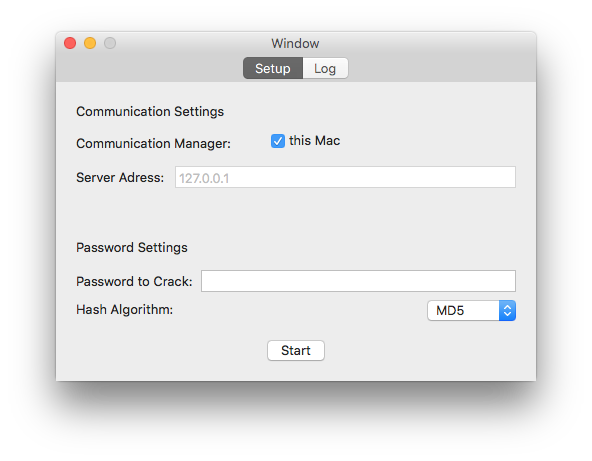
\includegraphics[natwidth=1200pt, natheight=349pt, width=0.6\textwidth]{images/WindowMaster.png}
		\caption{Benutzeroberfläche der implementierten Anwendung als Master der verteilten Anwendung}
	\label{fig:WindowMaster}
\end{figure}



\begin{figure}[!ht]
	\centering
		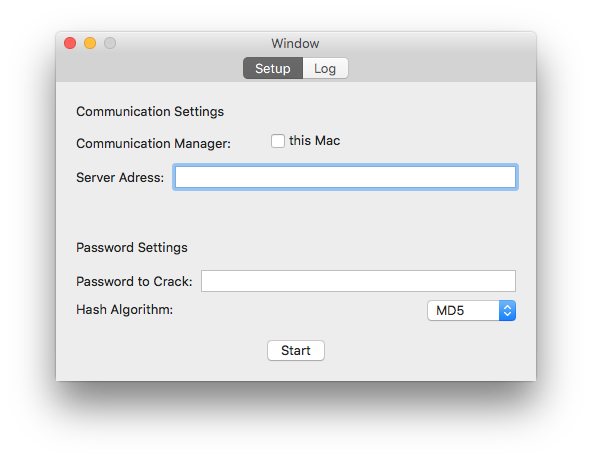
\includegraphics[natwidth=1200pt, natheight=349pt, width=0.6\textwidth]{images/WindowWorker.png}
		\caption{Benutzeroberfläche der implementierten Anwendung als Worker der verteilten Anwendung}
	\label{fig:WindowMaster}
\end{figure}

%TODO Screenshot von den Charts bzw. der Auswertung des Angriffs
